\chapter{Validating workflows for structural predictions of conjugated polymers with \texttt{espaloma}-parameterized forcefields}
The following chapter contains yet to be published work written by me with the guidance of Dr. Eric Jankowski. The following work will be submitted to the International Journal of Molecular Sciences. 
\label{chap:EspVal}
\section{Summary} 
Organic semiconductors are potentially useful building blocks for making new advanced materials, but predicting their stable morphologies is computationally challenging. Available forcefields may not sufficiently specify the interactions between the molecules' atoms, because prior work may not sufficiently specify the details of prior simulations, and because the simulations themselves must overcome kinetic barriers to self-assembly. We develop computational workflows for screening the morphologies of macromolecules and copolymers. We employ the \texttt{espaloma} toolkit to parameterize all-atom forcefields, \texttt{signac-flow} to manage simulation workspaces, \texttt{MoSDeF} tools to initialize simulation volumes, and \texttt{HOOMD-Blue} to perform molecular dynamics simulations. We compare morphologies predicted using our workflows to prior work using the \texttt{OPLS-UA} forcefield for perylene and poly-3-hexylthiophene (P3HT). We find that after resolving chemical ambiguities in molecular topologies, \texttt{espaloma} generates parameterizations that are similar to \texttt{GAFF}, and both the morphologies and temperature-density dependence of phase match prior work. We conclude that \texttt{espaloma} offers promise in the automated screening of molecules from more complex chemical spaces.

\section{Introduction}

Photovoltaic (PV) devices are one solution to potentially increasing the sustainable production of energy from the sun. To reduce the atmospheric carbon dioxide concentrations it is imperative that we increase the energy produced by green sources and reduce the amount of energy produced by fossil fuels and natural gas. A direct comparison of the life-cycle green-house gas (GHG) emissions for PV devices, natural gas and coal can be found in \autoref{tab:co2emissions}
\begin{table}[h]
    \centering
    \begin{tabular}{ll}
            \textbf{Method of Energy Production} & \textbf{GHG Emissions (g CO\textsubscript{2 eq}/kWh)} \\
    \hline
         \textbf{Solar}         &   124 \\
         \textbf{Natural Gas}   &   440 \\
         \textbf{Coal}          &   1040\\ 
    \end{tabular}
    \caption{The mean life-cycle GHG emissions of energy produced by solar, natural gas and coal in units of grams of CO\textsubscript{2} equivalent per kilowatt-hour \citep{MEHEDI2022118918,ghg_emissions}.}
    \label{tab:co2emissions}
\end{table}
\par The investigation into PV devices has become a large area of interest over the last several decades due to their increasing power conversion efficiency (PCE) as well as their promising effects on GHG emissions \citep{MEHEDI2022118918, ghg_emissions}. Organic photovoltaic devices have not only shown a promising increase in PCE over the last decade, from 2.8\% in 2002 to nearly 20\% in 2024, but they have also exhibited a lower production cost in comparison to their inorganic counterparts \citep{sondergaard_roll--roll_2012,Basu2024,Wang2021,Schilinsky2002}. As discussed in previous chapters, the efficiency of the OPV device is directly related to the morphology of the active layer \citep{mazzio_future_2015}. It has been predicted that long-range order in the active layer can provide higher charge carrier mobility, and therefore higher device PCE. Investigating the OPV molecules that have led to increased PCE's and the morphologies in which they self-assemble into is necessary to continuously improve the PCE of organic solar devices. Constraints in experimental research of OPV materials, such as cost and difficulty in structure determination, brings our attention to computational methods of studying OPV materials. The goal of this study has been to employ new a molecular dynamics framework to predict the morphologies of two OPV materials. We also compare the results of this framework to previous studies to ensure the accuracy of the predicted morphologies in efforts to validate the use of \texttt{espaloma} for OPV materials in our framework \citep{wang_end--end_2022}. MD simulations are a computational investigative technique that are founded on Newton's laws of motion. We use MD simulations to gain insight on how particles/molecules of interest interact over time to self assemble into equilibrated morphologies. A schematic of the MD workflow we implemented in this work is shown in \autoref{MD-Diagram}. 

\begin{figure}
    \centering
    \includegraphics[width=.9\linewidth]{src/figures/FF_figs/MD_process.png}
    \caption{Depictions of our generalized molecular dynamics workflow. Step 1 shows the creation of an \texttt{mBuild Compound} from a SMILES string. In step 2 we create our simulation object using \texttt{flowerMD} and \texttt{PACKMOL}. We employ \texttt{espaloma} to parameterize our molecules in step 3 and write the forcefield file. In step 4 we initialize the \texttt{HOOMD-Blue} simulation and predict the morphology of our molecules.}
    \label{MD-Diagram}
\end{figure}
\par In order to model molecules computationally, we have to implement forcefields. Forcefields are computational models that store all the particle information in bond, angle, torsion/dihedral, and non-bonded parameters. Forcefields are often built around specific areas of study and are sometimes missing parameters needed to model new materials. For example, a commonly used forcefield the Optimized Potentials for Liquid Simulations (OPLS) forcefield has mainly been built around simulating hydrocarbons and proteins \citep{opls,ghahremanpour_refinement_2022}. When attempting to simulate OPV molecules that include sulfur atoms, such as P3HT, OPLS is missing the hydrogen-carbon-carbon-sulfur (H-C-C-S) dihedral parameters. In the past, when parameters are missing, they had to be calculated using quantum mechanics calculations and added to the existing forcefield. This was a taxing process due to the computational complexity of quantum calculations as well as the lack of process automation. In this study, we employ the software program \texttt{espaloma}. \texttt{Espaloma} is a new, open-source software that uses graph neural networks to perceive chemical environments in a molecular graph and predict molecular parameters \citep{wang_end--end_2022}. \texttt{Espaloma} was designed for the investigation of biopolymers and has been used to accurately simulate them \citep{shirts2023, takaba_machine-learned_2024}.  For the use of organic, highly conjugated polymers, however, we must further analyze the results given from \texttt{espaloma} to ensure accurate parameterization. Using these \texttt{espaloma} generated forcefields we are able to parameterize and initialize simulations of materials that were previously missing parameters, this is shown in Step 4 of \autoref{MD-Diagram}. This allows us to run simulations on materials that were previously unable to be modeled due to missing information. To ensure that these \texttt{espaloma} forcefields accurately parameterizes OPV materials it is necessary to compare the morphologies produced by simulations initialized with an \texttt{espaloma} generated forcefield to those produced with previously validated forcefields. 
\begin{figure}[hbt!]
    \centering
    \includegraphics[width=0.8\textwidth]{src/figures/FF_figs/P3HTandPerylene.png} % Replace 'example-image' with your image file name and path
    \caption{Diagram of perylene molecule (left) and poly-3-hexylthiophene (P3HT) monomer (right).}
    \label{per_p3ht_fig}
\end{figure}
\par In this study we will compare united-atom (UA) simulation results of perylene and P3HT of simulations initialized with \texttt{espaloma} generated forcefields (ESP-UA) for each molecule with simulations initialized with the united-atom Optimized Potentials for Liquid Simulations (\texttt{OPLS-UA}) forcefield \citep{opls,ghahremanpour_refinement_2022}. These molecules were chosen because they are well studied molecules with OPV properties as well as their similar chemical and structure components (such as the thiophene ring in P3HT) to other interesting OPV materials (\autoref{per_p3ht_fig}). To ensure a more comprehensive comparison we have also compare the ESP-UA, \texttt{OPLS-UA} and Generalized Amber ForceField (\texttt{GAFF}) parameters, directly \citep{gaff}. To validate the predicted morphologies and structures we have calculated the grazing incident x-ray scattering (GIXS) pattern, order parameter, and radial distribution function (RDF). Molecular simulations are dependent on the forcefield to retain all specific information about the particles we are modeling. Due to this, simulation results may vary significantly if the forcefield parameters differ between simulations. In this work we aim to determine how, if at all, the \texttt{espaloma} generated forcefields affect the simulation results of perylene and P3HT. 

\section{Methods}
\subsection{Forcefield File Generation}
In order to perform simulations of macromolecules we must have two things, the molecule we want to simulate and that molecule's specific forces. The molecule object itself tells the simulation engine what atoms we are simulating and what connectivity they have, while the molecule's forces are what govern the molecule's behavior, i.e. attractions, repulsions, velocities, etc. These forces are the bond, angle, dihedral, and nonbonded forces. Building the molecule object is generally straight forward, the only requirement is that it must be in a format that is compatible with whatever simulation engine is being utilized. In this study, we employed \texttt{HOOMD-Blue} as our simulation engine, so we used \texttt{mBuild} to create and save our molecules as mol2 files \citep{anderson_hoomd-blue_2020,cummings_opensource_2021, Klein_mbuild}. The second requirement, having the molecule's specific forces, has proven nontrivial. When modeling large molecules it is often found that some of the parameters needed to simulate the molecule will be unknown. In this case, the unknown parameters must be calculated. We have created a workflow that allows you to generate a forcefield file containing all the particle parameters needed to simulate a molecule, from an \texttt{mBuild Compound}, \autoref{esp_diagram}. This workflow fits into the overall MD workflow (Section 4.2, \autoref{MD-Diagram}) within Step 4. 
\begin{figure}
    \centering
    \includegraphics[width=1\linewidth]{src/figures/FF_figs/esp_fig.png}
    \caption{Schematic of \texttt{Espaloma} forcefield and \texttt{mBuild Compound} generation.}
    \label{esp_diagram}
\end{figure}
The general process of this workflow is: \textbf{(1)} convert the \texttt{mBuild Compound} that you want to simulate to an \texttt{openMM Molecule} object. It is necessary for the molecule to be in an \texttt{openMM Molecule} format in order for \texttt{espaloma} to be able to create a graph of the molecule. \textbf{(2)} Rebuild the missing bonds in the \texttt{openMM Molecule} using the \texttt{BondWalker} function (See \autoref{bond_walk}). \textbf{(3)} Run our \texttt{BondWalked} molecule through the \texttt{espaloma} software to get the forcefield parameters and write these parameters into a forcefield file that is compatible with our simulation engine using our xml writer function. \textbf{(4)} Use the atom labels given by \texttt{espaloma} to rename the atoms in our \texttt{mBuild Compound}. This last step ensures that the correct parameters will be applied to the corresponding atoms. 

With the functions we created the entire workflow described above can be completed within the following lines of code: 
\begin{lstlisting}[language=Python]
import mbuild as mb
from functions.Espaloma_Functions import build_polymer, 
    espaloma, build_chain
class P3HT(mb.Compound):
    def __init__(self):
        super(P3HT,self).__init__()
        self.add(mb.load("CCCCCCC1=C(SC(=C1))",smiles=True))
        self.bond_indices = [24,25]
xml_filepath = "Example.xml"
typed_filepath = "Example.mol2"
espaloma(MONOMER = P3HT(),
        XML_FILEPATH = xml_filepath,
        TYPED_FILEPATH = typed_filepath )
\end{lstlisting}
A full tutorial of \texttt{espaloma} forcefield and typed \texttt{mBuild Compound} generation can be found at github.com/madilynpaul/Espaloma-Validation. 

\begin{figure}[ht]
    \centering
    \includegraphics[width=0.7\linewidth]{src/figures/FF_figs/bondwalk_algorithm.png}
    \caption{Algorithm used by \texttt{BondWalker} Function. First, we assign bonds to satisfy the octets of the atoms, if the octets are not satisfied after bonds are added the bonds are removed and added in different placements. This continues until all atoms in the molecule have a satisfied octet}
    \label{bond_walk}
\end{figure}

\subsection{Molecular Dynamics}
MD simulations using \texttt{HOOMD-Blue} were run on perylene and P3HT at 12 statepoints each. All simulations were performed on the Fry high performance computing cluster at Boise State using NVIDIA P100 and V100 GPUs. The canonical NVT ensemble was used (number of particles (N), volume (V) and temperature (T) were all held constant). A Nose-Hoover thermostat was utilized to control the temperature and a two-step velocity-verlet integration of Newton's equations of classical motion was used to update particle position and velocities. The \texttt{flowerMD} software package was used as a workflow for initializing simulations using a custom xml-based forcefield \citep{Albooyeh2023, gmso}. The pair interaction forces for perylene and P3HT can be found in \autoref{sigma_epsilon_comparison_table}, where they are compared to the pair forces from the \texttt{OPLS-UA} forcefield and the \texttt{GAFF} forcefield. 
\begin{table}[b!]
    \centering
    \begin{tabular}{c c|c|c}
        \multicolumn{4}{c}{$\sigma$ (\AA)}        \\
        \hline
                    &   C1      &   C0      &   S       \\
        \hline
        \texttt{Espaloma}    &   3.481   &   3.380   &   3.564   \\
        \texttt{OPLS-UA}     &   3.436   &   3.905   &   3.436   \\
        \texttt{GAFF}        &   3.3997  &   3.3997  &   3.564 \\

        \multicolumn{4}{c}{$\epsilon$ (kJ/mol)}         \\
        \hline
        \texttt{Espaloma}    &   0.3635  &   0.4554  &   1.046   \\
        \texttt{OPLS-UA}     &   0.4602  &   0.7113  &   1.339   \\
        \texttt{GAFF}        &   0.3598  &   0.4577  &   1.046   \\
    \end{tabular}
    \caption{A comparison of the non-bonded particle parameters produced by \texttt{espaloma}, \texttt{OPLS-UA} and \texttt{GAFF}.}
    \label{sigma_epsilon_comparison_table}
\end{table}
\par We initialize our system using \texttt{PACKMOL}, this is done by adding our particles to a cubic simulation box with applied periodic boundary conditions \citep{martinez_p_2009}. The molecules undergo a "mixing" step at high temperatures (1653 K for P3HT and 696 K for perylene) for $5 \times 10^6$ timesteps to ensure random molecule distribution. The simulations then proceed at the set temperature until equilibrium is reached, then simulations are continued until at least 50 independent samples are gathered. The parameters that varied between the systems are listed below in \autoref{sim_parameters}. The chain length for P3HT was chosen to create consistency between this study and previous work reported by Miller et. al. in order to draw comparisons of the results \citep{miller_optimization_2018}. These statepoints were chosen as they display a well-distributed range of statepoints on a previously constructed phase diagram. Each temperature range encompasses the solid-liquid transition temperature of approximately 500 K and 550 K for P3HT and perylene, respectively. The density ranges were chosen with respect to previous MD studies as well as experimental thin-film studies for P3HT. We expected to observe various phases (ordered, liquid, vapor, non-ordered) over this range of statepoints. This has allowed us to compare transition points in order to validate the use of \texttt{espaloma} to generate UA-forcefields for OPV molecules.
\begin{table}
  \centering
  \begin{tabular}{c|c|c}
      & \textbf{P3HT} & \textbf{Perylene} \\
    \hline
    Temperature Range (K) & [60.4,304.4,427.7,608.9]& [49.8,248.8,497.7,746.5]\\
    \hline
    Density Range (g/mL) & [0.25,0.5,1.0] & [0.5,1.0,1.5]\\
    \hline
    N & 100 & 250 \\
    \hline
    dt & 0.0003 & 0.0001 \\
    \hline
    M (amu) & 32.06 & 12.011 \\
    \hline
    \(\sigma\) (\AA)& 3.56 & 3.40 \\
    \hline
    \(\epsilon\) (kJ/mol)& 1.046 & 0.360\\
    \hline
    N\textsubscript{monomers}& 15 & 1 \\
  \end{tabular}
  \caption{A list of statepoints used in the P3HT and perylene simulations as well as the base units for each simulation (\begin{math}\sigma , \epsilon , M\end{math}).}
  \label{sim_parameters}
\end{table}

\subsection{Morphology Characterization}
\par Each equilibrated simulation has been characterized by grazing-incident x-ray scattering (GIXS) patterns. The GIXS patterns were generated using Freud's diffraction module \citep{freud2020}. The k-vector axis has been converted from reduced units to inverse angstroms (\AA\textsuperscript{-1}). The diffraction patterns have also been time-averaged over the last 20 independent snapshots of the simulation. Independent samples are determined by calculating the decorrelation time of each data set and excluding the data that is determined to be correlated to each other. 
\par The order parameter data was calculated by calculating the geometric centers of each molecule of perylene and each monomer of P3HT. Normal vectors to the molecular planes were used to determine the alignment of molecules, if the molecules planes were within a set angle range and if the molecules were within a certain distance from one another, they would be considered to be a part of the same cluster. The number of clusters were then tabulated and the order parameter was calculated by determining what percentage of molecules belong to a cluster, if all the molecules are found to be in the same cluster the order parameter, \begin{math}(\psi)\end{math}, is equal to 1. The code used to generate these figures can be found at github.com/madilynpaul/Espaloma-Validation. The geometric center of perylene was calculated using the whole molecule, while the geometric center of P3HT was calculated by only taking into account the thiophene ring in each monomer, excluding the aliphatic side chains. A depiction of the geometric centers used for both perylene and P3HT can be found in \autoref{fig:p3ht_per_CG}.

\begin{figure}
    \centering
    \includegraphics[width=1\linewidth]{src/figures/FF_figs/per_p3ht_CG.png}
    \caption{Example CG bead mapping overlayed with atomistic molecules for P3HT and perylene. Polymer with 3 repeating units used as example for P3HT for better visualization.}
    \label{fig:p3ht_per_CG}
\end{figure}

\par The radial distribution function (RDF) was calculated using the coarse-grained systems, shown in \autoref{fig:p3ht_per_CG}, to model how the molecule centers are distributed after equilibrium is achieved. The RDF’s are calculated using the Freud RDF module \citep{freud2020}. They were averaged over the last 20 independent samples for each system to ensure significant statistical sampling.

\section{Results and Discussion}

\subsection{Perylene}

\begin{figure}[ht]
    \centering
    \includegraphics[width=0.8\textwidth]{src/figures/FF_figs/PerylenePD.png} % 
    \caption{Temperature vs density clustering order parameter ($\Psi$) phase diagram of perylene at 12 statepoints.}
    \label{per_phase_diagram}
\end{figure}

\par \autoref{per_phase_diagram} shows the phase diagram of perylene as a function of temperature and density. The order parameter was calculated using the Freud cluster module with an angle cutoff of 10 degrees and distance cutoff of 6 \AA, scaled by the reference length of each simulation \citep{freud2020}. The phase transitions observed across the density axis are consistent with previously reported phase diagrams. At the lower temperatures we observe a transition from highly ordered to less ordered as the density increases. This is due to the steric hindrance of having a high number of molecules in a restricted volume. At higher temperatures, however, we observe an increase in order as we increase the density, this is also explained by the restricted volume, at a high temperature of 500 K and 750 K the molecules have enough thermal energy to overcome some steric hindrance and become more ordered than the lower temperature, but not enough space to become gaseous. We also observe a temperature dependent phase transition from well-ordered (solid) to liquid at approximately 300 K at both 0.5 g/mL and 1.0 g/mL. 

\begin{wrapfigure}{r}{0.5\textwidth}
  \begin{center}
    \includegraphics[width=0.48\textwidth]{src/figures/FF_figs/per_snapshot.png}
  \end{center}
  \caption{Snapshot of perylene taken from the most ordered morphology at a density of 0.5 g/mol and temperature of 248.8 K.}
  \label{Per_snapshot}
\end{wrapfigure}

\setlength{\parindent}{0cm}
While we observe reasonable results for the order parameter trends, the temperatures that these phase transitions occur at are approximately half of what we expect to observe from experiment and previous simulations. This contrast in transition temperatures can be explained by the difference in the epsilons that \texttt{Espaloma} provides in comparison to the \texttt{OPLS-UA} epsilons used to simulate perylene in the past study. This issue can be solved via epsilon scaling. The most ordered structure (T = 250 K, $\rho$ = 0.5 g/mL) exhibits significant \si{\pi}-stacking, which is very visible in \autoref{Per_snapshot}. 
\setlength{\parindent}{.6cm}
\begin{figure}[hbt!]
    \centering
    \includegraphics[width=.8\textwidth]{src/figures/FF_figs/per_GIXS.png} % Replace 
    \caption{Grazing incident x-ray scattering pattern of Perylene generated from an ESP-UA morphology in comparison to one generated from an \texttt{OPLS-UA} morphology. \texttt{OPLS-UA} GIXS pattern published by Miller, et. al. at Ref \citep{miller_enhanced_2017}.}
    \label{Per_GIXS}
\end{figure}
The GIXS pattern for perylene was generated from the most ordered morphology at a temperature of 250 K and density of 0.5 g/mol. Peaks are observed along both the x and y axes indicating significant long range order and hexagonally close packed columns, which are observed in \autoref{Per_snapshot}. Peak location and intensity align well with the GIXS scattering pattern published by Miller et al.~ \citep{miller_enhanced_2017}. The published GIXS pattern was generated from a perylene morphology predicted using OPLS-UA and was reported to align well with simulation results from Ref. \citep{Ishii}. 
\begin{figure}[ht!]
    \centering
    \includegraphics[width=1\textwidth]{src/figures/FF_figs/per_rdf.png} % Replace 'example-image' with your image file name and path
    \caption{Radial distribution function (RDF) of Perylene at various temperatures at a density of 0.5g/mL generated from an ESP-UA predicted morphology (left). RDF of perylene in various phases generated from an \texttt{OPLS-UA} predicted morphology (right). OPLA-UA RDF published by Miller, et al.~ at Ref \citep{miller_enhanced_2017}.}
    \label{per_rdf}
\end{figure}
The RDF of perylene at a density of 0.5 g/mL (\autoref{per_rdf}) shows a steep peak at ~1.1$\sigma$, corresponding to the hexagonal close packing observed in the morphologies at 50 K and 249 K. A comparison to the rdf reported in Miller, et al.~ at density of 1.7 g/mL shows impressive alignment of peak locations. Differences in peak intensity can be explained by the difference in density between the two systems. As expected, the RDFs calculated  at higher temperatures show less intense peaks. We observe high ordering at 50 K and 249 K, in correspondence to the RDF reported by Miller, et al.~ We observe consistent RDF peak locations between the EUA-simulation results at temperature of 498 K and the \texttt{OPLS-UA} simulation results reported in the droplet phase by Miller, et al.~ 
\subsection{Poly-3-Hexylthiophene (P3HT)}
\begin{figure}[hbt!]
    \centering
    \includegraphics[width=0.9\textwidth]{src/figures/FF_figs/P3HT_PD.png} % Replace 'example-image' with your image file name and path
    \caption{Temperature vs density clustering order parameter ($\Psi$) phase diagram of P3HT at 12 statepoints.}
    \label{p3ht_phase_diagram}
\end{figure}
\par \autoref{p3ht_phase_diagram} shows the clustering order parameter ($\Psi$) phase diagram of P3HT as a function of temperature and density. The order parameter was calculated using the Freud cluster module  with an angle cutoff of 10 degrees and distance cutoff of 6 \AA, scaled by the reference length of each simulation. As observed with perylene, the transition temperatures are off by a factor of two from our previously simulated results with \texttt{OPLS-UA} as the forcefield. Again, this can be explained by the differences in epsilons between the ESP-UA forcefield and OPLA-UA forcefield, (difference can be found in \autoref{sigma_epsilon_comparison_table}). \texttt{Espaloma} reports an epsilon of 0.4554 kJ/mol for the aliphatic side chain carbons of P3HT, while \texttt{OPLS-UA} uses an epsilon of 0.7113 kJ/mol. This creates more ordered side chains in the \texttt{OPLS-UA} simulations in comparison to the \texttt{espaloma} simulations. This observation is supported by the work in Reference \citep{marsh_controlling_2014}, stating that the lower the epsilon for side chains of P3HT monomers we observe lamellar structures at lower temperatures than if the epsilon was higher \citep{marsh_controlling_2014}. 
\begin{figure}[h!]
    \centering
    \includegraphics[width=.9\textwidth]{src/figures/FF_figs/p3htGIXS&exp.png} % Replace 'example-image' with your image file name and path
    \caption{Grazing Incident X-ray Scattering Pattern of P3HT at 0.5 g/$cm^3$ and 304 K with corresponding experimental scattering pattern published by Ko, et al.~ at Ref \citep{p3ht_experimental}. Copyright 2012 American Chemical Society}
    \label{p3ht_GIXS}
\end{figure}
\par The GIXS scattering pattern of the most ordered structure (0.5 g/$cm^3$, 304 K) displays significant correlation to the experimental scattering pattern of P3HT (\autoref{p3ht_GIXS}). Peaks are observed at approximately 1.65 \AA \textsuperscript{-1} corresponding to the (010) plane as well as peaks along the (100) plane spaced approximately 0.3 \AA \textsuperscript{-1} apart. This correlation between experiment and simulation confirms that the \texttt{espaloma}-generated forcefield files are responsibly parameterizing and representing the P3HT polymer in simulation. The lamellar structure that is represented by the scattering pattern in \autoref{p3ht_GIXS} is shown in \autoref{p3ht_lamellar}. 
\begin{figure}[hbt!]
    \centering
    \includegraphics[width=0.6\textwidth]{src/figures/FF_figs/p3ht_0.5den_2.42kT.png}
    \caption{Snapshot of P3HT's most ordered morphology at a density of 0.5 g/mol and temperature of 304.4 K.}
    \label{p3ht_lamellar}
\end{figure}
\par \autoref{P3HT RDF} shows the radial distribution function of ESP-UA P3HT (left) and OPLS-UA P3HT (right). The ESP-UA RDF was generated at a temperature of 304 K and a density of 0.5g/m. Three vertical dashed lines in the ESP-UA RDF correspond to the local maxima and minima highlighted in the OPLS-UA RDF. The first peak in each corresponds to the aligned $\pi$-stacking of the thiophene rings, shown in \autoref{P3HT RDF}a. The second peak aligns with the anti-aligned $\pi$-stacking of the thiophene rings, shown in \autoref{P3HT RDF}b. The OPLS-UA RDF was calculated using the geometric center of thiophene ring, shown in \autoref{P3HT RDF}c. The ESP-UA RDF was calculated using only the S-S interactions, excluding those in the same chain. The sulfurs were chosen for the ESP-UA RDF because they are central to the ring, hold the most mass and have the largest radius. 
\begin{figure}[hbt!]
    \centering
    \includegraphics[width=1\textwidth]{src/figures/FF_figs/p3ht_rdf.png} % Replace 'example-image' with your image file name and path
    \caption{Radial distribution function (RDF) of P3HT at a temperature of 304 K and a density of 0.5g/mL generated from an ESP-UA predicted morphology (left). RDF of P3HT generated from an \texttt{OPLS-UA} predicted morphology (right). OPLA-UA RDF published by Miller, et al.~ at Ref \citep{miller_optimization_2018}.}
    \label{P3HT RDF}
\end{figure}

\par 
In comparison to other forcefield techniques \texttt{espaloma} appears to generate reasonable constraints. The forcefield constraints generated by \texttt{espaloma} are similar, if not exact, to those found in the generalized amber force field (\texttt{GAFF}). \autoref{sigma_epsilon_comparison_table} shows the comparison of \texttt{espaloma} generated sigmas and epsilon values for the main atom types in perylene and P3HT. The \texttt{ESP-UA} parameters stray from the \texttt{OPLS-UA} parameters, but the similarity of the simulation results for \texttt{ESP-UA} and \texttt{OPLS-UA} leads us to conclude that \texttt{ESP-UA} parameterizes perylene and P3HT as accurately as \texttt{OPLS-UA} and that these differences in pair forces do not significantly influence the predicted morphologies. One difficulty that emerged while implementing \texttt{espaloma} into our simulation workflow was that we also employ the Molecular Simulation Design Framework (\texttt{MoSDeF}) \citep{cummings_opensource_2021}. A straight forward way to insert \texttt{espaloma} into the into the \texttt{MoSDeF} framework while using \texttt{HOOMD-Blue} as the simulation engine did not exist. To implement \texttt{espaloma} it was necessary to create a pipeline to ensure compatibility between the \texttt{mBuild Compounds}, which are necessary to create our simulation object, and the \texttt{OpenFF Molecule} objects which \texttt{espaloma} needs in order to generate the forcefield parameters. When creating this pipeline we needed to ensure that we could convert \texttt{mBuild Compounds} to \texttt{OpenFF Molecules} and then convert the \texttt{OpenFF Molecules} back to \texttt{mBuild} molecules while retaining the atom-type labels that \texttt{espaloma} has generated for each atom. Because \texttt{espaloma} creates a unique forcefield for each molecule, it also generates atom types for each atom in our molecule. There is no straight conversion from \texttt{mBuild} to \texttt{OpenFF}, so in order to do this conversion we must have a "stepping stone" which has a direct conversion to and from both \texttt{OpenFF Molecule} objects and \texttt{mBuild Compound} objects. While there are many molecule types that fit this constraint, they must also conserve the atom indexing when converting from the \texttt{OpenFF Molecule} object to the \texttt{mBuild Compound}. This is necessary to retain the atom-type information. In order to apply the \texttt{espaloma} generated forcefield file to our simulation object, the atoms in the simulation object need to match the naming in the forcefield file. This is necessary for \texttt{espaloma} generated forcefield files because they currently do not include \texttt{SMARTS} strings in order to determine the atom type of each atom in the molecule.
\section{Conclusions}
\par We have successfully validated and implemented \texttt{espaloma} into a \texttt{MoSDeF} workflow for investigating OPV materials via MD simulations. \texttt{Espaloma} generates reasonable forcefield parameters for macromolecules with high aromaticity as well as for thiophene-based conjugated polymers. The forcefield parameters predicted by \texttt{Espaloma} were similar to \texttt{GAFF} parameters and predicted morphologies that aligned well with morphologies predicted using \texttt{OPLS-UA} forcefields. The GIXS scattering patterns for both perylene and P3HT showed long range order that was consistent with published experimental and theoretical results. RDF peak locations confirmed that the espaloma generated forcefields were responsibly and accurately modeling both molecules of interest. The order parameter trends were consistent with published results for perylene and P3HT, but had inconsistent transition temperatures. Future simulations with scaled epsilons must be conducted to confirm if this is a result of epsilon differences between the \texttt{OPLS-UA} model and the \texttt{ESP-UA} model. From these results we confidently conclude that \texttt{Espaloma} accurately parameterized conjugated macromolecules and polymers and present a cohesive workflow for implementing \texttt{espaloma} into a \texttt{HOOMD-Blue} and \texttt{MoSDeF} based molecular dynamics investigations. 